%amsart class
\documentclass[a4paper, 10pt, reqno]{amsart}

%Packages
\usepackage[utf8]{inputenc}
\usepackage[english]{babel}
\usepackage{graphics}
\usepackage{physics}
\usepackage{listings}
\usepackage{hyperref}
\usepackage{blindtext}
\usepackage{xcolor}
\usepackage{subcaption}
\usepackage{pgf}
\usepackage{tikz}
\usepackage{tikzscale}
\usepackage{pgfplots}
\usepackage{placeins}
\usepackage{parskip}

\hypersetup{colorlinks=true, linkcolor=black, citecolor=black,
urlcolor=blue}
%\hypersetup{hidelinks}

\pgfplotsset{compat=1.5}
\newlength\figureheight
\newlength\figurewidth
\setlength\figurewidth{0.98\textwidth}
\setlength\figureheight{0.75\figurewidth}
\captionsetup[subfigure]{width=0.9\textwidth}

\usepackage{etoolbox}
\makeatletter
\patchcmd{\@maketitle}
  {\ifx\@empty\@dedicatory}
  {\ifx\@empty\@date \else {\vskip3ex
  \centering\footnotesize\@date\par\vskip1ex}\fi
   \ifx\@empty\@dedicatory}
  {}{}
\patchcmd{\@adminfootnotes}
  {\ifx\@empty\@date\else \@footnotetext{\@setdate}\fi}
  {}{}{}
\makeatother

%Custom colors
\definecolor{code}{rgb}{0.9, 0.17, 0.31}
\definecolor{coolgrey}{rgb}{0.55, 0.57, 0.67}
\definecolor{cyan(process)}{rgb}{0.0, 0.72, 0.92}
\definecolor{lightwhite}{rgb}{0.9647058823529412, 0.9647058823529412, 0.9647058823529412}
\definecolor{royalblue}{rgb}{0.25, 0.41, 0.88}
\definecolor{mediumseagreen}{rgb}{0.24, 0.7, 0.44}
%listing customization
\lstset{ %
  backgroundcolor=\color{lightwhite},
  basicstyle=\ttfamily\footnotesize,        % the size of the fonts that are used for the code
  breakatwhitespace=true,         % sets if automatic breaks should only happen at whitespace
  breaklines=true,                 % sets automatic line breaking
  captionpos=b,                    % sets the caption-position to bottom
  commentstyle=\color{mediumseagreen},    % comment style
  deletekeywords={...},            % if you want to delete keywords from the given language
  escapeinside={\%*}{*)},          % if you want to add LaTeX within your code
  extendedchars=true,              % lets you use non-ASCII characters; for 8-bits encodings only, does not work with UTF-8
  frame=single,	                   % adds a frame around the code
  keepspaces=true,                 % keeps spaces in text, useful for keeping indentation of code (possibly needs columns=flexible)
  keywordstyle=\color{code},       % keyword style
  language=[90]Fortran,                 % the language of the code
  otherkeywords={...},           % if you want to add more keywords to the set
  emph={get_H_p, spline, exp, abs, sqrt},
  emphstyle={\color{royalblue}},
  rulecolor=\color{white},         % if not set, the frame-color may be changed on line-breaks within not-black text (e.g. comments (green here))
  numbers=left,
  showspaces=false,                % show spaces everywhere adding particular underscores; it overrides 'showstringspaces'
  showstringspaces=false,          % underline spaces within strings only
  showtabs=false,                  % show tabs within strings adding particular underscores
  stepnumber=1,                    % the step between two line-numbers. If it's 1, each line will be numbered
  tabsize=3,	                   % sets default tabsize to 2 spaces
}

%Frontpage stuff
\title[Milestone 3]{\Large{Milestone 3: The evolution of structures in the universe} \\
\normalsize{AST5220 - Cosmology 2}}

\author[San]{Metin San}

\date{\today}



%Begining document
\begin{document}

\maketitle
\begin{center}
   \vspace*{-0.6cm} \textsc{\url{https://github.com/MetinSa/AST5220/tree/master/milestone2}}
\end{center}

\begin{abstract}
We compute the evolution of density perturbations, $\delta, \delta_b$, and their velocities, $v, v_b$ for dark matter and baryons during the history of the Universe. Additionally we compute the evolution of the gravitational potentals $\Phi$ and $\Psi$, along with the temperature fluctuations of the photons $\Theta$. We observe a strong trend in the evolution of these quantities where they are greatly affected by the change in cosmological epochs. In the early universe, when modes are far outside the horizon, $k\eta \ll 1$, all quantities are mostly constant. The amplitudes then experience a scale dependant growth/decline upon horizon entry, which is suppressed during the radiation dominated eta, $a \ll a_\mathrm{eq}$. The quantities again experience a change in behaviour when the universe enters the matter dominated era , $a \gg a_\mathrm{eq}$, which lasts til until dark energy domination, $x \approx -1$. 
\end{abstract}

\section{Introduction}
This is the third out of four milestones on the path to computing the CMB power spectrum. In this milestone we will study and visualize how small fluctuations in the baryon-photon-dark-matter fluid grew shortly after inflation until today. We will do so by implementing and solving the linearized Boltzmann and Einstein equations, making use of routines developed in previous milestones. The main goal of this milestone is to compute two dimensional grids in both time and Fourier scale of a number of quantities of interest, along with their derivatives.

Similarly to Milestone 1, all programs used for the direct calculations are written in FORTRAN 90 and based on a provided skeleton code. The analysis of the results are done using Python. All tools and source code used to produce the results and figures can be found on my Github through the link below the author name on the front page.

The structure of the report consist of four individual sections. It begins with a theory section where we introduce and motivate the relevant physics that are used in the calculations. Following is a section where we discuss the numerical implementation and methods used to solve the Boltzmann and Einstein equations. We then present the results through figures and observational descriptions in a results section. The results are then discussed and interpreted in a discussion section. The report is finally concluded with a brief conclusion where we reflect back on the work done and the results achieved.

\section{Theory}
Similar to in Milestone 2, we will assume that the reader is familiar with the previously presented equations and definitions, meaning that we will refrain from redefining them here. As mentioned in the introduction, we are interested in a number of quantities. Here follows a short description off the most important quantities
\begin{itemize}
    \item $\Phi(x,k)$, $\Psi(x,k)$: Gravitational potentials (metric perturbations) with $\Psi$ corresponding to the Newtonian (time) potential, and $\Phi$ to a perturbation in the spatial curvature. The presence of $\Phi$ and $\Psi$ results in a cosmology that deviates from the homogeneous and flat FRW metric.
    \item $\delta(x,k)$, $\delta_b(x,k)$:  Dark matter and baryon density perturbations, describing overdensities in the otherwise mostly homogeneous density distribution.
    \item $v(x,k)$, $v_b(x,k)$: Radial velocity (collapse velocity) of the dark matter and baryons respectively, induced by the density perturbations through the continuity equation.
    \item $\Theta(x,k)$: Temperature perturbation in the photon distribution. Describes deviations from the mean temperature (anisotropies in temperature), and can be associated with $\delta T/T$.
\end{itemize}

The evolution of these quantities through out the history of the Universe is described by the the linear Einstein-Boltzmann equations. Deriving these is an extensive process which is why we will only present their final form here. These equations describe the evolution of perturbations in the universe, and their numerical solutions play a very central role in our understanding of cosmology. 

\subsection{The Einstein-Boltzmann Equations}
We will now present the solution to the linear Einstein-Boltzmann equations (without considering polarization or neutrinos). The temperature perturbations evolve as
\begin{align}
    \Theta_{0}^{\prime}= & -\frac{c k}{\mathcal{H}} \Theta_{1}-\Phi^{\prime},\label{eq: monopole'}\\
    \Theta_{1}^{\prime}= & \frac{c k}{3 \mathcal{H}} \Theta_{0}-\frac{2 c k}{3 \mathcal{H}} \Theta_{2}+\frac{c k}{3 \mathcal{H}} \Psi+\tau^{\prime}\left[\Theta_{1}+\frac{1}{3} v_{b}\right],\label{eq: dipole'}\\
    \Theta_{l}^{\prime}= & \frac{l c k}{(2 l+1) \mathcal{H}} \Theta_{l-1}-\frac{(l+1) c k}{(2 l+1) \mathcal{H}} \Theta_{l+1}+\tau^{\prime}\left[\Theta_{l}-\frac{1}{10} \Theta_{l} \delta_{l, 2}\right], \quad 2 \leq l<l_{\max }, \label{eq: multipole'}\\
    \Theta_{l}^{\prime}= & \frac{c k}{\mathcal{H}} \Theta_{l-1}-c \frac{l+1}{\mathcal{H} \eta(x)} \Theta_{l}+\tau^{\prime} \Theta_{l}, \quad l=l_{\max }\label{eq: multipole' final}
\end{align}
where $\Theta_0, \Theta_1, ... ,\Theta_l$ are the monopole, dipole, and the higher order multipoles expansions of the photon temperature perturbations. The prime denotes the change with respect to the variable $x$,  $\prime = d/dx$, with $k$ being the Fourier transform of $x$. 

The gravitational potentials in the perturbed metric $\Psi$ and $\Phi$ evolve on the following forms
\begin{align}
   \Phi^{\prime} = & \Psi-\frac{c^{2} k^{2}}{3 \mathcal{H}^{2}} \Phi+\frac{H_{0}^{2}}{2 \mathcal{H}^{2}}\left[\Omega_{m} a^{-1} \delta+\Omega_{b} a^{-1} \delta_{b}+4 \Omega_{r} a^{-2} \Theta_{0}\right], \label{eq: Phi'} \\ 
   \Psi = &-\Phi-\frac{12 H_{0}^{2}}{c^{2} k^{2} a^{2}} \Omega_{r} \Theta_{2}. \label{eq: Psi'}
\end{align}

The velocities $v$, and $v_b$ along with their derivatives are given as
\begin{align}
    v^{\prime}= & -v-\frac{c k}{\mathcal{H}} \Psi, \label{eq: v'}\\
    v_{b}^{\prime}= & -v_{b}-\frac{c k}{\mathcal{H}} \Psi+\tau^{\prime} R\left(3 \Theta_{1}+v_{b}\right) , \label{eq: v_b'}
\end{align}
where $ R = 4\Omega_r/3\Omega_b a$.

Furthermore we have the evolution of the dark matter and baryon perturbations $\delta^\prime$ and $\delta_{b}^\prime$ given as
\begin{align}
    \delta^{\prime}= & \frac{c k}{\mathcal{H}} v-3 \Phi^{\prime}, \label{eq: delta}\\
   \delta_{b}^{\prime}= & \frac{c k}{\mathcal{H}} v_{b}-3 \Phi^{\prime}. \label{eq: delta_b}
\end{align}

We observe that all these equations take the form of differential equations that are tightly coupled to each other, and will therefore have to be solved simultaneously.

\subsection{Initial Conditions}
In order to start solving the Einstein-Boltzmann equations we first need the initial conditions of the Universe. We start by observing that all the equations are depending on $\Phi$. We can therefore chose $\Phi = 1$ which then acts as a normalization for all the initial conditions. This does not imply that perturbation $\Phi$ of the gravitational field is equal to 1, but rather that all the other initial conditions are normalized to the value of $\Phi$ at $x = x_i$.

With this convention, the initial conditions read
\begin{align} 
    \Phi = & 1, \\
    \delta = & \delta_{b} = \frac{3}{2} \Phi, \\ 
    v = & v_{b} = \frac{c k}{2 \mathcal{H}} \Phi, \\
    \Theta_{0} = & \frac{1}{2} \Phi, \\
    \Theta_{1} = &-\frac{c k}{6 \mathcal{H}} \Phi, \\
    \Theta_2 = & - \frac{20 c k}{45 \mathcal{H} \tau^\prime} \Theta_1,\\
    \Theta_{l}= &-\frac{l}{2 l+1} \frac{c k}{\mathcal{H} \tau^{\prime}} \Theta_{l-1}.
\end{align}

\subsection{Tight Coupling Regime}
At very early times in the history of the Universe the optical depth, $\tau$, is very large as a result of a tight coupling between photons and baryons. This means that the electrons in the hot fluid only ever interact with their closest neighbors. As a result, the temperature fluctuations are smoothed. The only relevant fluctuations in this regime are therefore the monopole, $\Theta_0$ as it measures the temperature at the electron position, the dipole, $\Theta_1$ which as a result of the Doppler effect is given as the velocity of the fluid, and the quadrupole $\Theta_2$ which provides the polarization signal. We can therefore set the higher-ordered photon moments during this time to their initial conditions
\begin{align}
    \Theta_{2}= & -\frac{20 c k}{45 \mathcal{H} \tau^{\prime}} \Theta_{1},\\
    \Theta_{l}= & -\frac{l}{2 l+1} \frac{c k}{\mathcal{H} \tau^{\prime}}
    \Theta_{l-1}.
\end{align}

\section{Implementation}
The implementation for Milestone 3 consists of completing the module \textbf{evolution\_mod.f90} and also some slight adjustments to \textbf{time\_mod.f90} which we made in Milestone 1.

\subsection{Code Structure}
We start by creating a quadratic $k$ array that corresponds to different scale sizes. The perturbation arrays corresponding to their respective scale size are then initialized. The goal is to study the evolution of these quantities all the way from inflation today, meaning that we need a time grid ($x$) which runs from inflation and until today. This is achieved by altering the time grid made in Milestone 1 slightly by including another 1000 grid points spaced between $x_\mathrm{init} = \log a_\mathrm{init}$ and until $x_\mathrm{rec}$, where $a_\mathrm{init} = 10^{-8}$ and $x_\mathrm{rec}$ are the previous starting times of the time array (start of recombination). 

The next step is to integrate the set of equations for all times $x$ and all scales $k$. Since our equations are given by slightly different expressions depending on the era, we split the integration process into two parts. The first part considers the set of equation during the tight coupling regime, where we only consider moments up to $\Theta_2$ as the higher moments are suppressed. We define the tight coupling era to end when one of the following conditions are fulfilled: $\tau^\prime < 10$, or $ck/\mathcal{H}\tau^\prime > 0.1$ or when we enter recombination $x > x_\mathrm{rec}$. Before the integration starts, we use a individual subroutine to extract $x_{\mathrm{tc}}$, the tight coupling time.

The second section considers the era from tight coupling until today. Here we use the standard set of equations, meaning that we have to compute all moments up to $l = 6$. The integration in both parts are done using the odeint routine previously discussed. We have created two individual subroutines for each era which computes the derivatives that are to be used in the odeint routine. This is done to both increase the clarity of the code and to ease implementation. This does however results in a lot of duplicate code as most of the equations are the same in both era. 

\subsection{Tight Coupling Stability}
As previously mentioned, in the tight coupling regime $\tau$ is very large. This can quickly lead to computational problems in the the $(\Theta_1 + v_b)$ term in equation \eqref{eq: v_b'} as even a tiny numerical error in $\Theta_1$ will result in disastrous errors in $\Theta_1'$ and $v_b'$, leaving our set of differential equations unstable in this period as they are heavily coupled.

We will solve this problem by expanding $(\Theta_1 + v_b)$ in powers of $1/\tau'$. Doing so and playing around with the equations results in the following new expressions for $\Theta_{1}^\prime$ and $v_{b}^\prime$ which we will need to use during this era

\begin{align} 
    q = & \frac{-\left[(1-2 R) \tau^{\prime}+(1+R) \tau^{\prime \prime}\right]\left(3 \Theta_{1}+v_{b}\right)-\frac{c k}{\mathcal{H}} \Psi+\left(1-\frac{\mathcal{H}^{\prime}}{\mathcal{H}}\right) \frac{c k}{\mathcal{H}}\left(-\Theta_{0}+2 \Theta_{2}\right)-\frac{c k}{\mathcal{H}} \Theta_{0}^{\prime}}{(1+R) \tau^{\prime}+\frac{\mathcal{H}^{\prime}}{\mathcal{H}}-1} \\ 
    v_{b}^{\prime} = & \frac{1}{1+R}\left[-v_{b}-\frac{c k}{\mathcal{H}} \Psi+R\left(q+\frac{c k}{\mathcal{H}}\left(-\Theta_{0}+2 \Theta_{2}\right)-\frac{c k}{\mathcal{H}} \Psi\right)\right] \\ \Theta_{1}^{\prime} = &\frac{1}{3}\left(q-v_{b}^{\prime}\right) 
\end{align}

\section{Results}
We will now present the results of the milestone. We have chosen to include the following physical quantities as our results: $\Phi$, $\Psi$, $\delta$, $\delta_b$, $v$, $v_b$, $\Theta_0$, and $\Theta_1$. These can be seen in the two figures \ref{fig: 1} and \ref{fig: 2}. A descriptive interpretation of the results can be found in the caption corresponding to each quantity. A more in depth discussion around the results is provided in the next section.

\begin{figure}
\makebox[\textwidth][c]{
  \begin{subfigure}[t]{0.7\textwidth}
    \centering
    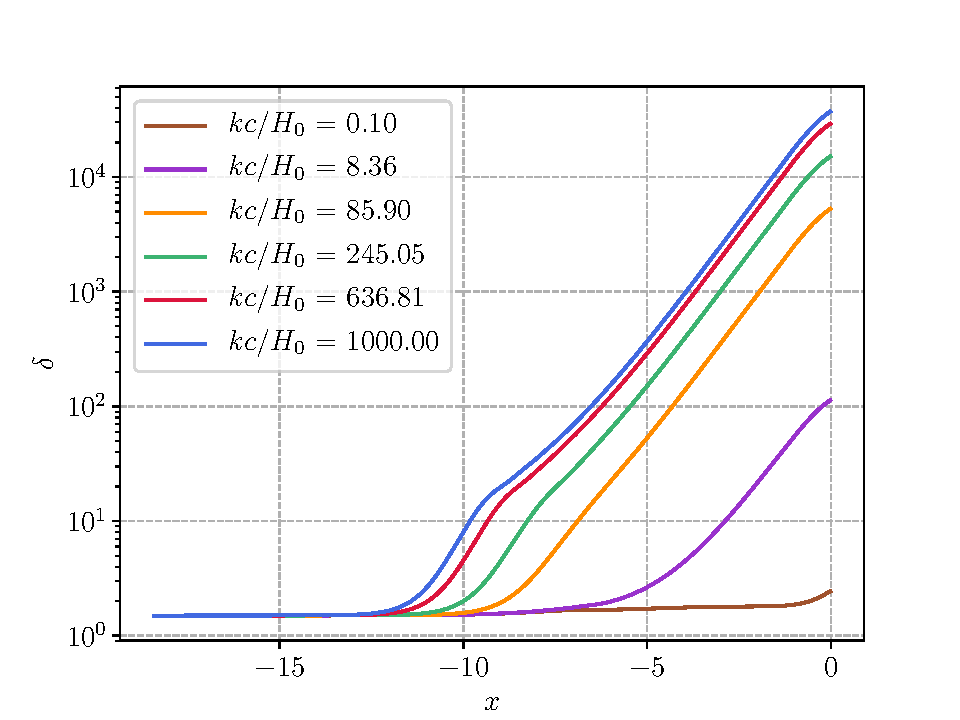
\includegraphics[width=0.9\textwidth]{figures/delta.pdf} 
    \caption{Dark matter density perturbations, $\delta$. We observe that the time at which the perturbations start to grow is scale dependant, where the small scales begin to grow at earlier times. For small (and some intermediate) scales, the strong initial growth of the perturbations experiences a slight suppression after horizon entry. This suppression seems to last until about recombination, after which the perturbations pick up the pace and continue to grow in a linear manner in log scale. The larger scales which enter the horizon at later times is unaffected by the suppression and grow mostly linear.} 
    \label{fig: 1a} 
  \end{subfigure}%% 
  \begin{subfigure}[t]{0.7\textwidth}
    \centering
    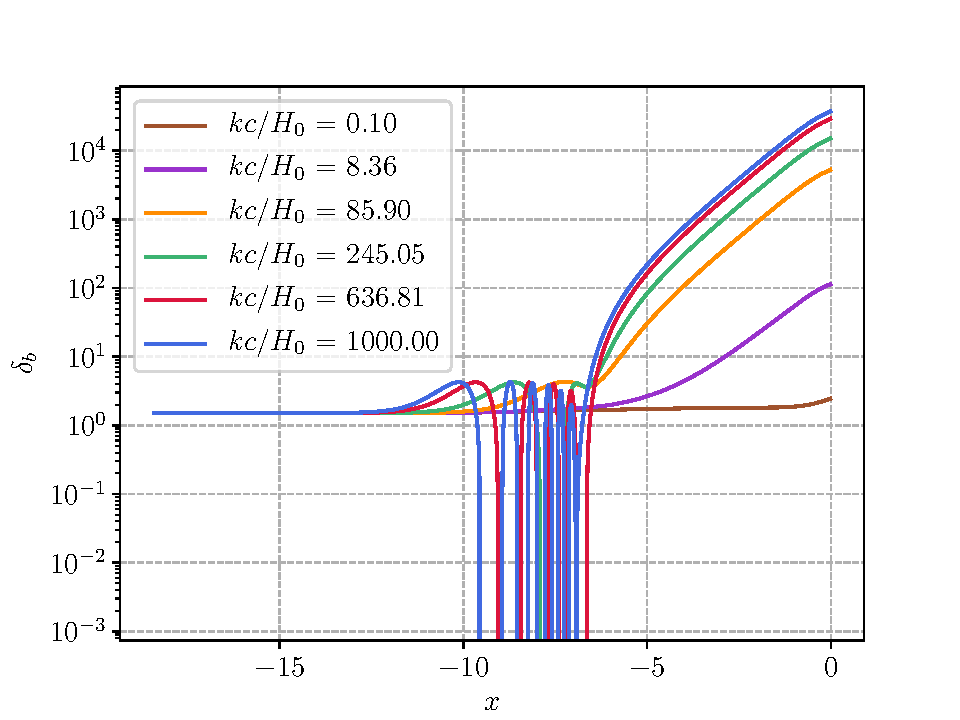
\includegraphics[width=0.9\textwidth]{figures/delta_b.pdf} 
    \caption{Baryon density perturbations, $\delta_b$. 
    Similar to the case with dark matter, the baryonic perturbations begin to grow prior to horizon entry at different times depending on the scale. However, in contrast to the slight suppression experienced by the dark matter after horizon entry, the baryonic perturbations experience a complete suppression (for small and some intermediate scales). This suppressing seems to last until recombination times, after which a quick growth makes the perturbations follow the evolution of the dark matter.} 
    \label{fig: 1b} 
  \end{subfigure} 
  }
  \makebox[\textwidth][c]{
  \begin{subfigure}[t]{0.7\textwidth}
    \centering
    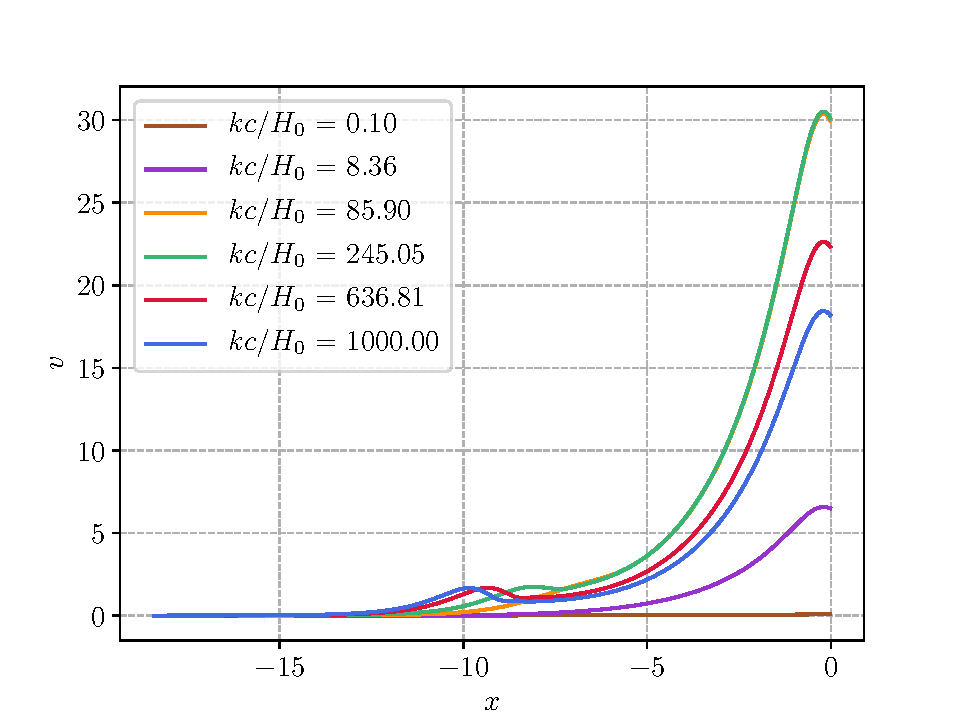
\includegraphics[width=0.9\textwidth]{figures/v.pdf} 
    \caption{Average radial velocity of dark matter, $v$. A small bump in velocity is observed for small scales (and some intermediate) at times of horizon entry which suppresses the velocity. After the initial suppression, the velocities see an exponential like growth which seemingly starts at around recombination. They then continue to grow until they reach a maximum at around $x \approx -1$. Similar to the density contrast, the values of the velocities are scale dependant, with the intermediate scales experience the largest velocities while the large scales experience next to non.} 
    \label{fig: 1c} 
  \end{subfigure}%%
  \begin{subfigure}[t]{0.7\textwidth}
    \centering
    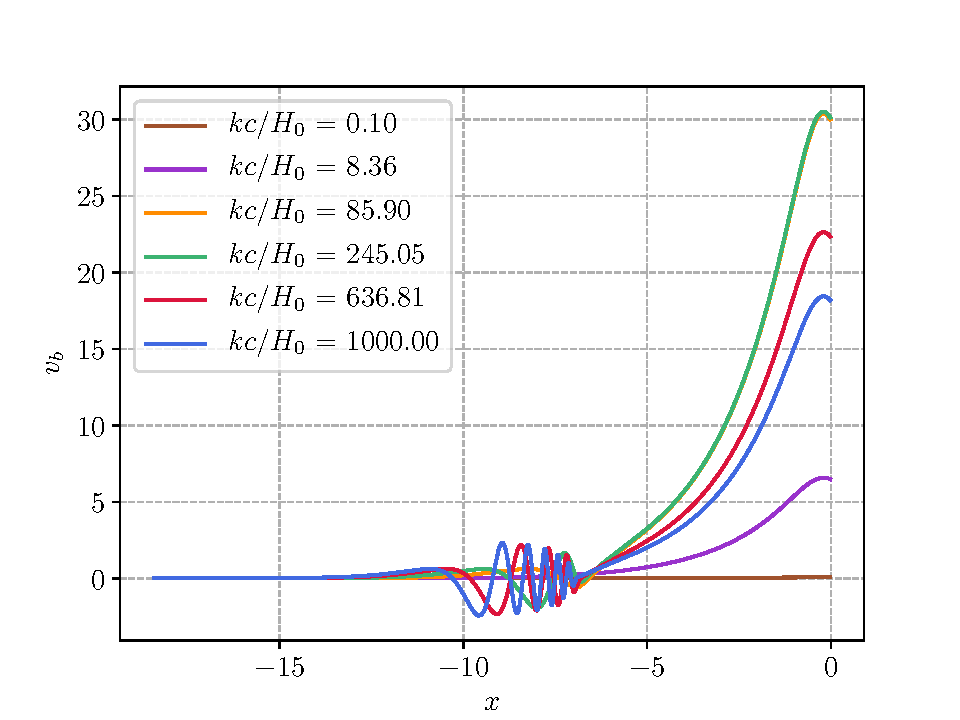
\includegraphics[width=0.9\textwidth]{figures/v_b.pdf} 
    \caption{Average radial velocity for baryons, $v_b$. We observe an interesting behaviour after horizon entry for the small and intermediate scales. Unlike the dark matter which was slightly suppressed, the baryons at the small and intermediate scales oscillate around $v_b = 0$ in a damping manner. The smallest scales experience the most oscillations, while the largest do not experience any. These oscillations continue until around recombination times, after which all scales follow the dark matter evolution. } 
    \label{fig: 1d} 
  \end{subfigure} 
  }
  \caption{Figures showing the time evolution of the dark matter and baryon density perturbations and velocities, $\delta$, $\delta_b$, $v$, and $v_b$. All physical quantities as plotted as a function of $x$, and is shown for six different values of $k$. These scales are chosen so that all three main regimes are shown; large-scales (small values of $k$), intermediate scales (intermediate values of $k$), and small scales (large values of $k$).}
  \label{fig: 1} 
\end{figure}

\begin{figure}
\makebox[\textwidth][c]{
  \begin{subfigure}[t]{0.7\textwidth}
    \centering
    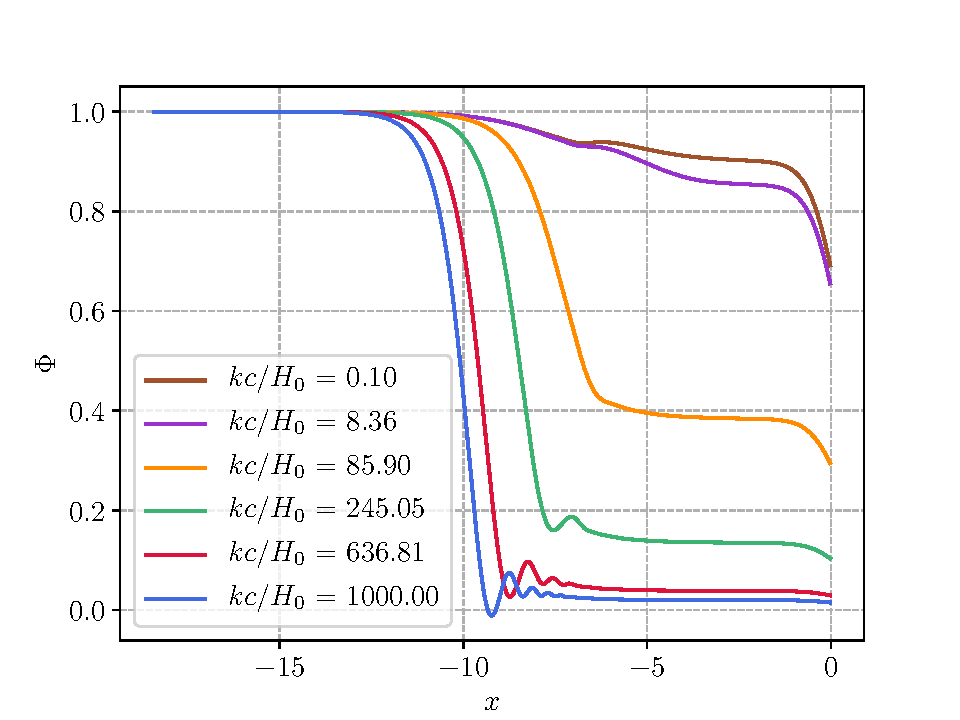
\includegraphics[width=0.9\textwidth]{figures/Phi.pdf} 
    \caption{Gravitational potential $\Phi$ (Time). We observe that the potential for small and intermediate scales experiences a quick drop in value after inflation. The quick decrease comes to an abrupt end after horizon entry, at which the potential oscillates in a damping manner around some final value which depends on the scale. The smallest scales experience the most oscillations while the large scales don't oscillate at all. Large scales never experience the early drop, and remains close to its initial value of $\Phi = 1$. Similar to the other quantities the potential drops in value at around $x \approx -1$, which is most notably for the large scales.} 
    \label{fig: 2a}
  \end{subfigure}%% 
  \begin{subfigure}[t]{0.7\textwidth}
    \centering
    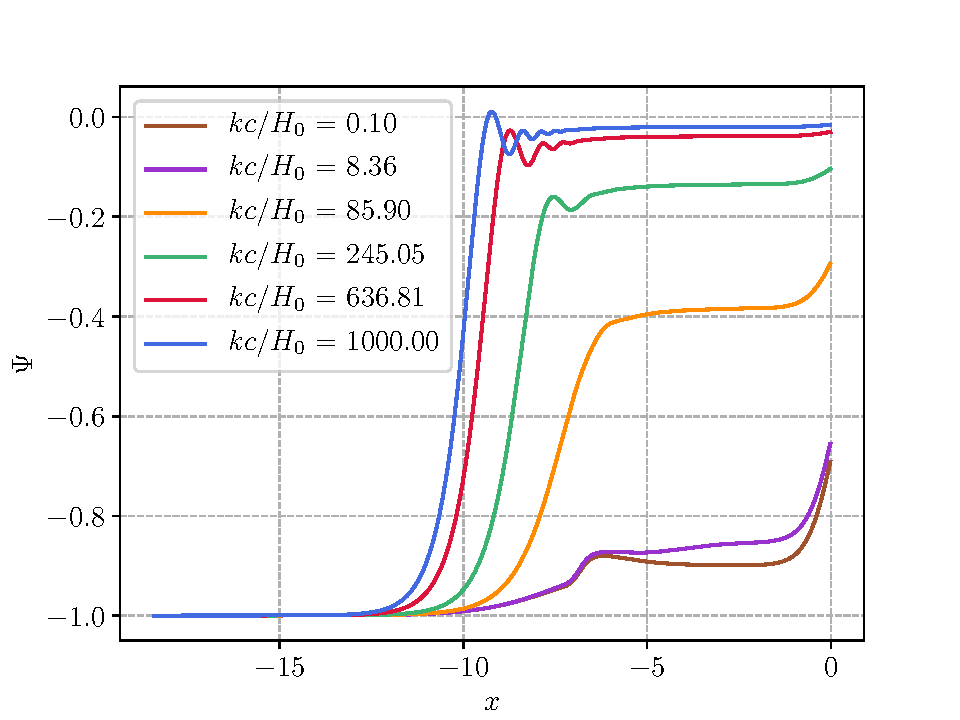
\includegraphics[width=0.9\textwidth]{figures/Psi.pdf}
    \caption{Gravitational potential $\Psi$ (Spatial curvature). The potential appears to trace $\Phi$ as its negative for the entire evolution, meaning that all observations are mirrored about $x = 0$. }
    \label{fig: 2b} 
  \end{subfigure} 
  }
  \makebox[\textwidth][c]{
  \begin{subfigure}[t]{0.7\textwidth}
    \centering
    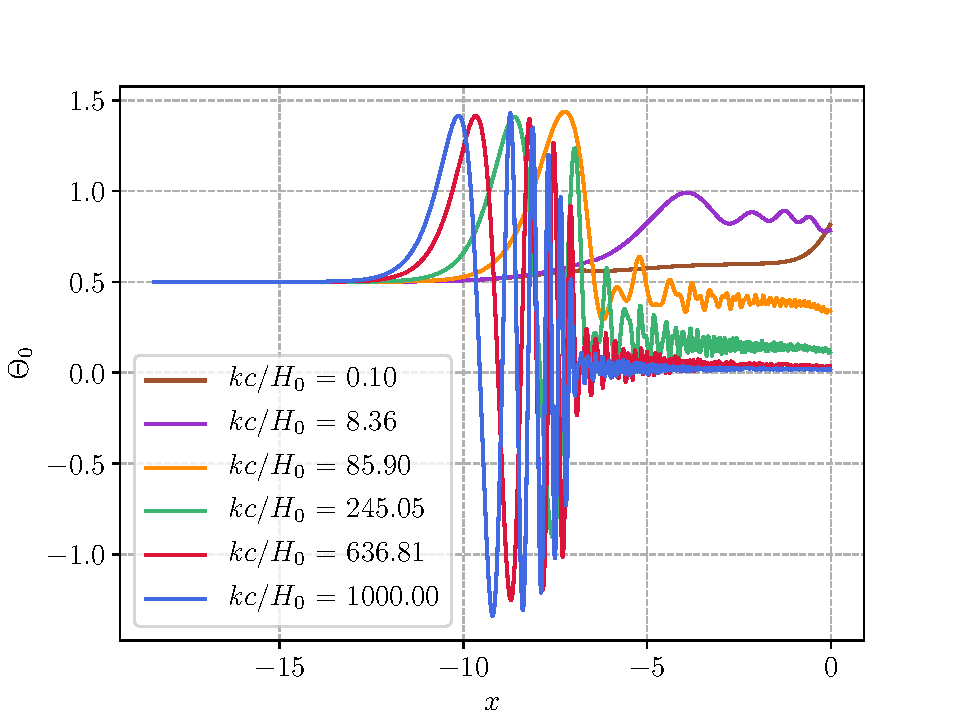
\includegraphics[width=0.9\textwidth]{figures/Theta0.pdf}
    \caption{Monopole in temperature fluctuation $\Theta_0$. We observe that small and intermediate scales all grow to approximately the same value of $\Theta_0$ around times of horizon entry. They proceed to quickly drop and oscillate around their final value which is scale dependant. After recombination, this oscillation is heavily damped, after which the small and intermediate scales mimic a converging damped harmonic oscillator. The small scales converge towards $\Theta_0 \approx 0$, while the intermediate and larger scales retain a non-zero fluctuations today. } 
    \label{fig: 2c} 
  \end{subfigure}%%
  \begin{subfigure}[t]{0.7\textwidth}
    \centering
    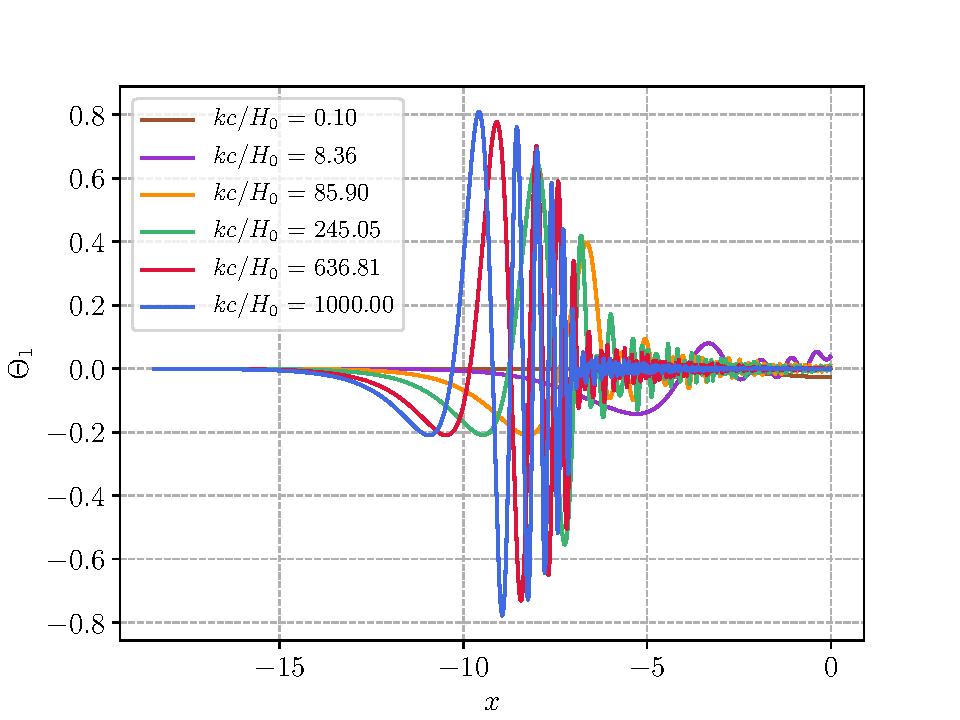
\includegraphics[width=0.9\textwidth]{figures/Theta1.pdf}
    \caption{Dipole in temperature fluctuation $\Theta_1$. The dipole displays a similar behaviour to the monopole with the exception that all scales converge and oscillate about $\Theta_1 = 0$. Again, we observe that the smallest scales experience the most frequent oscillations. } 
    \label{fig: 2d} 
  \end{subfigure} 
  }
  \caption{Figures showing the time evolution of the the two gravitational potentials $\Phi$ and $\Psi$, and the two first multipoles of the temperature fluctuations $\Theta_0$ and $\Theta_1$. The plots follow the same format as the figures in \ref{fig: 1}, and the same six scale magnitudes are used.}
  \label{fig: 2} 
\end{figure}

\section{Discussion}
We will now dive deeper into the results and try to interpret and understand why they appear as they do.

\subsection{Density perturbations and velocities}
The dark matter density perturbations seen in figure \ref{fig: 1a} seems to be in accordance with our expectations. We know from perturbation theory that an overdensity $\delta$ at some scale will grow roughly as $\delta \propto a^2$ after inflation. After the overdensity enters the horizon, the perturbation is suppressed to a growth of $\delta \propto \log a$ as a result of the universe being radiation dominated. This is known as the Meszaros effect, and it continues until matter-radiation equality which occurred at roughly the same time as recombination (we will refer to matter-radiation equality, $x_{\mathrm{eq}}$, as "recombination"), after which the perturbation continues growing at a rate of $\delta \propto a$. This is only relevant for the smallest scales and some intermediate as the other scales cross the horizon at post radiation dominated eras.

In the baryonic perturbation scenario in figure \ref{fig: 1b} we observe a much stronger suppression after horizon entry and until recombination. This is because the baryons have intrinsic motion, in contrast to the cold dark matter which only responds to gravity. During this era, the Universe is radiation dominated and the baryons are locked in a single hot fluid together with the CMB photons. The pressure in the photon-baryon fluid is enormous relative to its density. The pressure attempts to equalize it self with the surroundings while gravity wants to increase the overdensity, resulting in oscillations about small overdensities and no overall growth. This is known as the baryonic acoustic oscillations as these oscillations resulted in sound waves propagating through the Universe which will leave their mark on the final power spectrum.

A common theme through out our results is that perturbations grow prior to horizon crossing. After horizon entry the perturbations are suppressed, and the strength and type of suppression depends on on the quantity (baryonic or dark matter) and scale. This is a result of the quantities being heavily coupled. In the case of the dark matter velocities in figure \ref{fig: 1c}, the Meszaros suppression of the overdensity slows the velocities down during the radiation dominated era. In the case of the baryon velocity in figure \ref{fig: 1d}, the aforementioned acoustic oscillations are clearly visible as we observe the baryons oscillate about $v_b = 0$ with negative velocities being interpreted as the pressure pushing back the collapsing perturbation back.

\subsection{Gravitational potentials}
From figure \ref{fig: 2a} we observe that the gravitational potential $\Phi$ quickly drops for the small and intermediate modes that enter the horizon. For large scales we observe little to no change as these scales only enter the horizon in a post radiation dominated era. These scales only change slightly around recombination times. The small oscillations that are present at the smallest scales are likely connected to baryonic acoustic oscillations combating gravity. Once matter and radiation is decoupled, the potential remains mostly constant. We do however observe that the potential drops for all scales at $x \approx -1$. From Milestone 1, we know that this is the time where dark energy domination kicks in, meaning that this might be interpreted as the point where gravity loses the battle against the dark energy.

It can be shown that to the first order, the potential $\Psi$ can be approximated as $\Psi = -\Phi$. This is a very good approximation as there is no visible difference between the two plots in figures \ref{fig: 2a} and \ref{fig: 2b} (except for the mirroring). A comparison shows that the only difference between the two potentials occur during recombination but this is only a difference to the third digit. However, we do include the additional term in \eqref{eq: Psi'} as even very small errors may result in large errors later when we attempt to compute the power spectrum in the coming milestone.

\subsection{Temperature fluctuations}
As previously mentioned in the theory section, the monopole describes the deviation from the mean temperature at the location of the electron which emitted the CMB photon. It is therefore natural to think that it would follow the evolution the density perturbations of the baryons, which it clearly does. The temperature fluctuates the largest during the radiation dominated era within the horizon which is expected from the density behaviour. It should be noted that a warmer photon corresponds to a patch on the CMB which has a weaker gravitational field, since the photon loses energy as it climbs out of the field. The monopole value being scale dependant is interesting and might be a result of general smoothing on different scales.

The dipole is strongly connected to the dopplershift of the photons, meaning that its strongly velocity correlated. As expected, it varies the strongest during the baryonic acoustic oscillations and converges to $\Theta_1 = 0 $ as $ x \rightarrow 0$.

\section{Conclusion}
To conclude the discussion; We observe a strong trend through out our results. The evolution of the different quantities are heavily epoch dependant, with horizon entry and matter-radiation equality being the two main evolution defining eras. We also find that the scale of the observed modes are highly significant as large-scale modes evolve in a very different manner than the small-scale modes for large parts of the Universes history.

The obtained results seem consistent with theory and our cosmological knowledge as we are able to both recognize, and understand the behaviors of the quantities for the most part. This suggests that our code is well functioning, and we are ready to take on the final milestone where we will utilize the infrastructure from milestones 1 through 3 to compute the CMB power spectrum.



\nocite{*}
\bibliography{references}{}
\bibliographystyle{plain}
\end{document}